
\chapter{GCSE Transformation Questions}
\begin{enumerate}
  \item \mbox{}
  \begin{figure}[H]
    \centering
    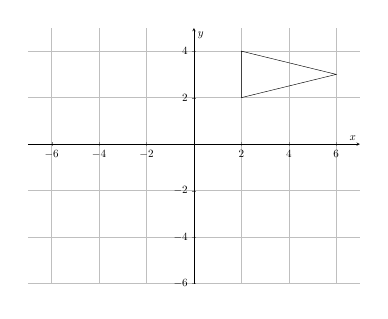
\begin{tikzpicture}[scale = 0.4]
      \begin{axis}[
          xmin = -7, xmax = 7,
          ymin = -6, ymax = 5,
          grid = both,
          axis lines = middle,
          width = \textwidth,
          height = 0.8\textwidth,
          xlabel = {$x$},
          ylabel = {$y$},
        ]
        \draw (2,2) -- (2,4) -- (6,3) -- (2,2);
        \end{axis}
      \end{tikzpicture}
    \end{figure}
    On the grid, enlarge the triangle by scale factor $-\frac{1}{2}$, centre $(0, -2)$.\mrk{2}
    \item \mbox{}
    \begin{figure}[H]
      \centering
      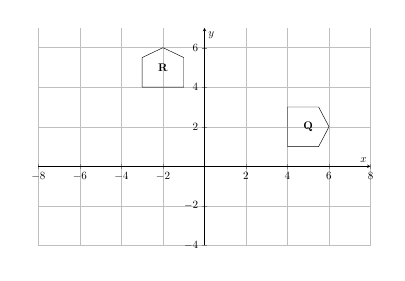
\begin{tikzpicture}[scale = 0.4]
        \begin{axis}[
            xmin = -8, xmax = 8,
            ymin = -4, ymax = 7,
            grid = both,
            axis lines = middle,
            width = \textwidth,
            height = 0.7\textwidth,
            xlabel = {$x$},
            ylabel = {$y$},
          ]
          \draw (-3,4) -- (-3,5.5) -- (-2,6) -- (-1,5.5) -- (-1,4) -- (-3,4);
          \draw (4,1) -- (4,3) -- (5.5,3) -- (6,2) -- (5.5,1) -- (4,1);
          \node at (-2,5) {\textbf{R}};
          \node at (5,2) {\textbf{Q}};
          \end{axis}
        \end{tikzpicture}
      \end{figure}
      Describe fully the single transformation that maps shape \textbf{Q} onto shape \textbf{R}.\mrk{3}\\
      \tikz\draw[thick, dashed] (0,0) -- (0.9\textwidth,0);\\
      \tikz\draw[thick, dashed] (0,0) -- (0.9\textwidth,0);\\
      \tikz\draw[thick, dashed] (0,0) -- (0.9\textwidth,0);
      \item \mbox{}
      \begin{figure}[H]
        \centering
        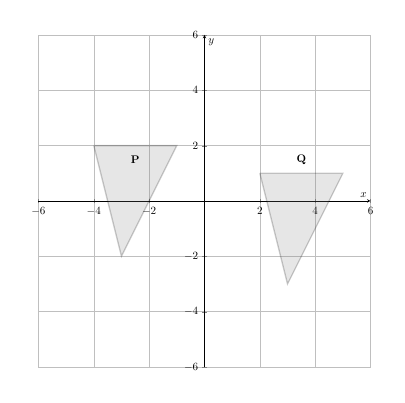
\begin{tikzpicture}[scale=0.4]
          \begin{axis}[
              xmin = -6, xmax = 6,
              ymin = -6, ymax = 6,
              grid = both,
              axis lines = middle,
              width = \textwidth,
              height = \textwidth,
              xlabel = {$x$},
              ylabel = {$y$},
            ]
            \filldraw[color=black, fill=gray, opacity=0.2, very thick] (-4,2) -- (-1,2) -- (-3,-2) -- (-4,2);
            \filldraw[color=black, fill=gray, opacity=0.2, very thick] (2,1) -- (5,1) -- (3,-3) -- (2,1);

            \node at (-2.5,1.5) {\textbf{P}};
            \node at (3.5,1.5) {\textbf{Q}};
            \end{axis}
          \end{tikzpicture}
        \end{figure}
        Describe fully the single transformation that maps triangle \textbf{P} onto triangle \textbf{Q}.\mrk{2}\\
        \tikz\draw[thick, dashed] (0,0) -- (0.9\textwidth,0);\\
        \tikz\draw[thick, dashed] (0,0) -- (0.9\textwidth,0);
\end{enumerate}